\input{HTTP_Transfer_commands.tex}
\question[5] In einer Webseite sind zwei Bilder eingebettet.
Die Webseite hat eine Größe von \sizeweb. Das erste Bild umfasst \sizepa, das zweite Bild \sizepb.
Server und Client verwenden persistentes HTTP, aber ohne Pipelining. Es steht eine stabile Datenrate von \rate{} zur Verfügung. Die Round Trip Time zwischen Server und Client beträgt \rtt. Nach der Übertragung des zweiten Bildes beendet der Client die Verbindung.

Skizzieren Sie ein Sequenzdiagramm des Kommunikationsablaufs und notieren Sie jeweils die Zeiten in Millisekunden, gerundet auf eine Stelle nach dem Komma, wann die einzelnen HTTP Antworten vollständig beim Client angekommen sind.
\begin{solutionbox}{15cm}

		\tikzset{%
			msg/.style={midway,fill=white,align=center,font=\tiny},
			}
		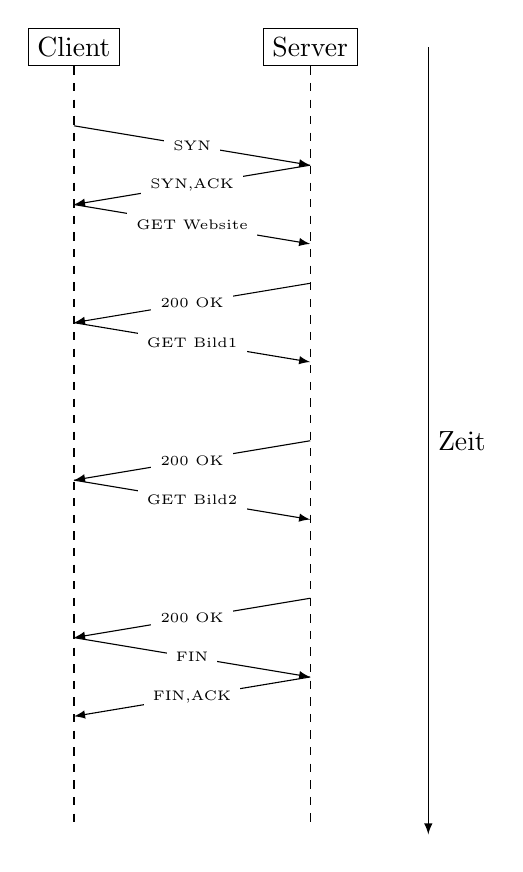
\begin{tikzpicture}
			\node[draw] (bt) at (0,0) {Client};
			\node       (bb) at (0,-10) {};
			\node[draw] (wt) at (3,0) {Server};
			\node       (wb) at (3,-10) {};
			\draw[dashed] (bt) -- (bb);
			\draw[dashed] (wt) -- (wb);
			\draw[-latex] (0,-1)   -- node[msg] {SYN} +(3,-.5);
			\draw[-latex] (3,-1.5) -- node[msg] {SYN,ACK} +(-3,-.5) node[left,font=\footnotesize]{\sola};
			\draw[-latex] (0,-2)   -- node[msg] {GET Website} +(3,-.5);
			\draw[-latex] (3,-3) -- node[msg] {200 OK} +(-3,-.5) node[left,font=\footnotesize]{\solb};
			\draw[-latex] (0,-3.5)   -- node[msg] {GET Bild1} +(3,-.5);
			\draw[-latex] (3,-5) -- node[msg] {200 OK} +(-3,-.5) node[left,font=\footnotesize]{\solc};
			\draw[-latex] (0,-5.5)   -- node[msg] {GET Bild2} +(3,-.5);
			\draw[-latex] (3,-7) -- node[msg] {200 OK} +(-3,-.5) node[left,font=\footnotesize]{\sold};
			\draw[-latex] (0,-7.5)   -- node[msg] {FIN} +(3,-.5);
			\draw[-latex] (3,-8) -- node[msg] {FIN,ACK} +(-3,-.5) node[left,font=\footnotesize]{\sole};
			\draw[-latex] (4.5,0) -- node[midway,right] {Zeit}(4.5,-10) ;
		\end{tikzpicture}
\end{solutionbox}
